%Correct the file name.
%X: book number
%Y: part number
%ZZZ: page number in three digits. So page 3 would be 003.

\documentclass[11pt]{amsbook}

\usepackage{../HBSuerDemir}	% ------------------------
\usepackage{wrapfig}

\begin{document}

% ++++++++++++++++++++++++++++++++++++++
\hPage{b2p1/165}
% ++++++++++++++++++++++++++++++++++++++
\begin{wrapfigure}{r}{0.30\textwidth}
    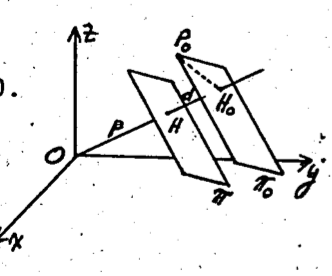
\includegraphics[width=0.30\textwidth]{images/b2p1-165-fig01}
\end{wrapfigure}
Indeed, let $\pi_{0}$ be the plane //$\pi$,passing through $P_{0}(x_{0},  y_{0}, z_{0})$:\\
$\pi_{0}$: x cos$\alpha$ + y cos$\beta$ + z cos$\gamma$ - (p$\pm$d)=0.\\
Since $P_{0}\epsilon\pi_{0}$,then \\
x$_{0}cos\alpha$ + y$_{0}cos\beta$ + z$_{0}cos\gamma$ - (p$\pm$d)=0\\
$\Rightarrow $ $\pm$d=x$_{0}cos\alpha$ + y$_{0}cos\beta$ + z$_{0}cos\gamma$ - p\\
$\Rightarrow $ d=$|$x$_{0}cos\alpha$ + y$_{0}cos\
\beta$ + z$_{0}cosr - $p$|$.
\\
\begin{exmp}Given the point A(3, -2, -1) and $\vec{N}$ = (1, -8, 4),
\begin{hEnumerateAlpha}
    \item Write the equation of the plane $\pi$ through A and perpendicular to $\vec{N}$,
    \item Obtain the normal equation of $\pi$,
    \item Find the distance of B(2, 2, -5) from $\pi$.
\end{hEnumerateAlpha}
\end{exmp}
\begin{hSolution}
\begin{hEnumerateAlpha}
   \item (x-3 - 8(y+2) +4(z+1) = 0\\
   $\Rightarrow$ x - 8y + 4z - 15 = 0
   \item Since $\sqrt{1^2 + (-8)^2 + 4^2}$ = 9, we have\\
   $\frac{x - 8y + 4z - 15}{9}$ = 0
   \item d(B, $\pi$) = $\frac{|2 - 8.2 + 4(-5) - 15|}{9}$ = 49/9
\end{hEnumerateAlpha}
\end{hSolution}
\begin{exmp} Given the planes\\
$\pi$: 2x - 2y + z - 3 = 0 and $\pi^\prime$: 4x - 4y + 2z + 7 = 0
\begin{hEnumerateAlpha}
\item show that $\pi$//$\pi^\prime$
\item find the distance d($\pi$, $\pi^\prime$)
\end{hEnumerateAlpha}
\end{exmp}
\begin{hSolution}
\begin{hEnumerateAlpha}
\item $\frac{2}{4} = \frac{-2}{-4}
=\frac{1}{2} \Rightarrow \pi//\pi^\prime$
\end{hEnumerateAlpha}
\end{hSolution}

% =======================================================
\end{document}  
